% vim:ft=tex:
%
\documentclass[]{beamer}

\usepackage[orientation=portrait,size=a1,scale=1.5,debug]{beamerposter}
\usepackage{subcaption}
%\usepackage[demo]{graphicx}

\mode<presentation>{\usetheme{usyd}}

\graphicspath{{figures/}}

\title{The Detection and Characterisation of \\\ \vspace{0.4em}\\ Molecular Crystals}
\author{Malcolm Ramsay and Peter Harrowell}
\institute{School of Chemistry, The University of Sydney}

\begin{document}
\begin{frame}[t]{}
  \begin{columns}[t]

    \begin{column}{0.45\linewidth}

      \begin{block}{Abstract}
        The wide range of crystal structures of a molecular crystal can make it difficult to detect and
        characterise all of them individually. We present a general approach to the detection and
        characterisation of local crystalline ordering using machine learning which can distinguish
        between crystal types and the liquid in excess of 95\% accuracy.
      \end{block}

      \begin{block}{Introduction}
        The molecule we are studying has three crystal structures with nearly equivalent energies.
        \begin{figure}[h]
          \centering
          \begin{subfigure}[t]{0.3\linewidth}
              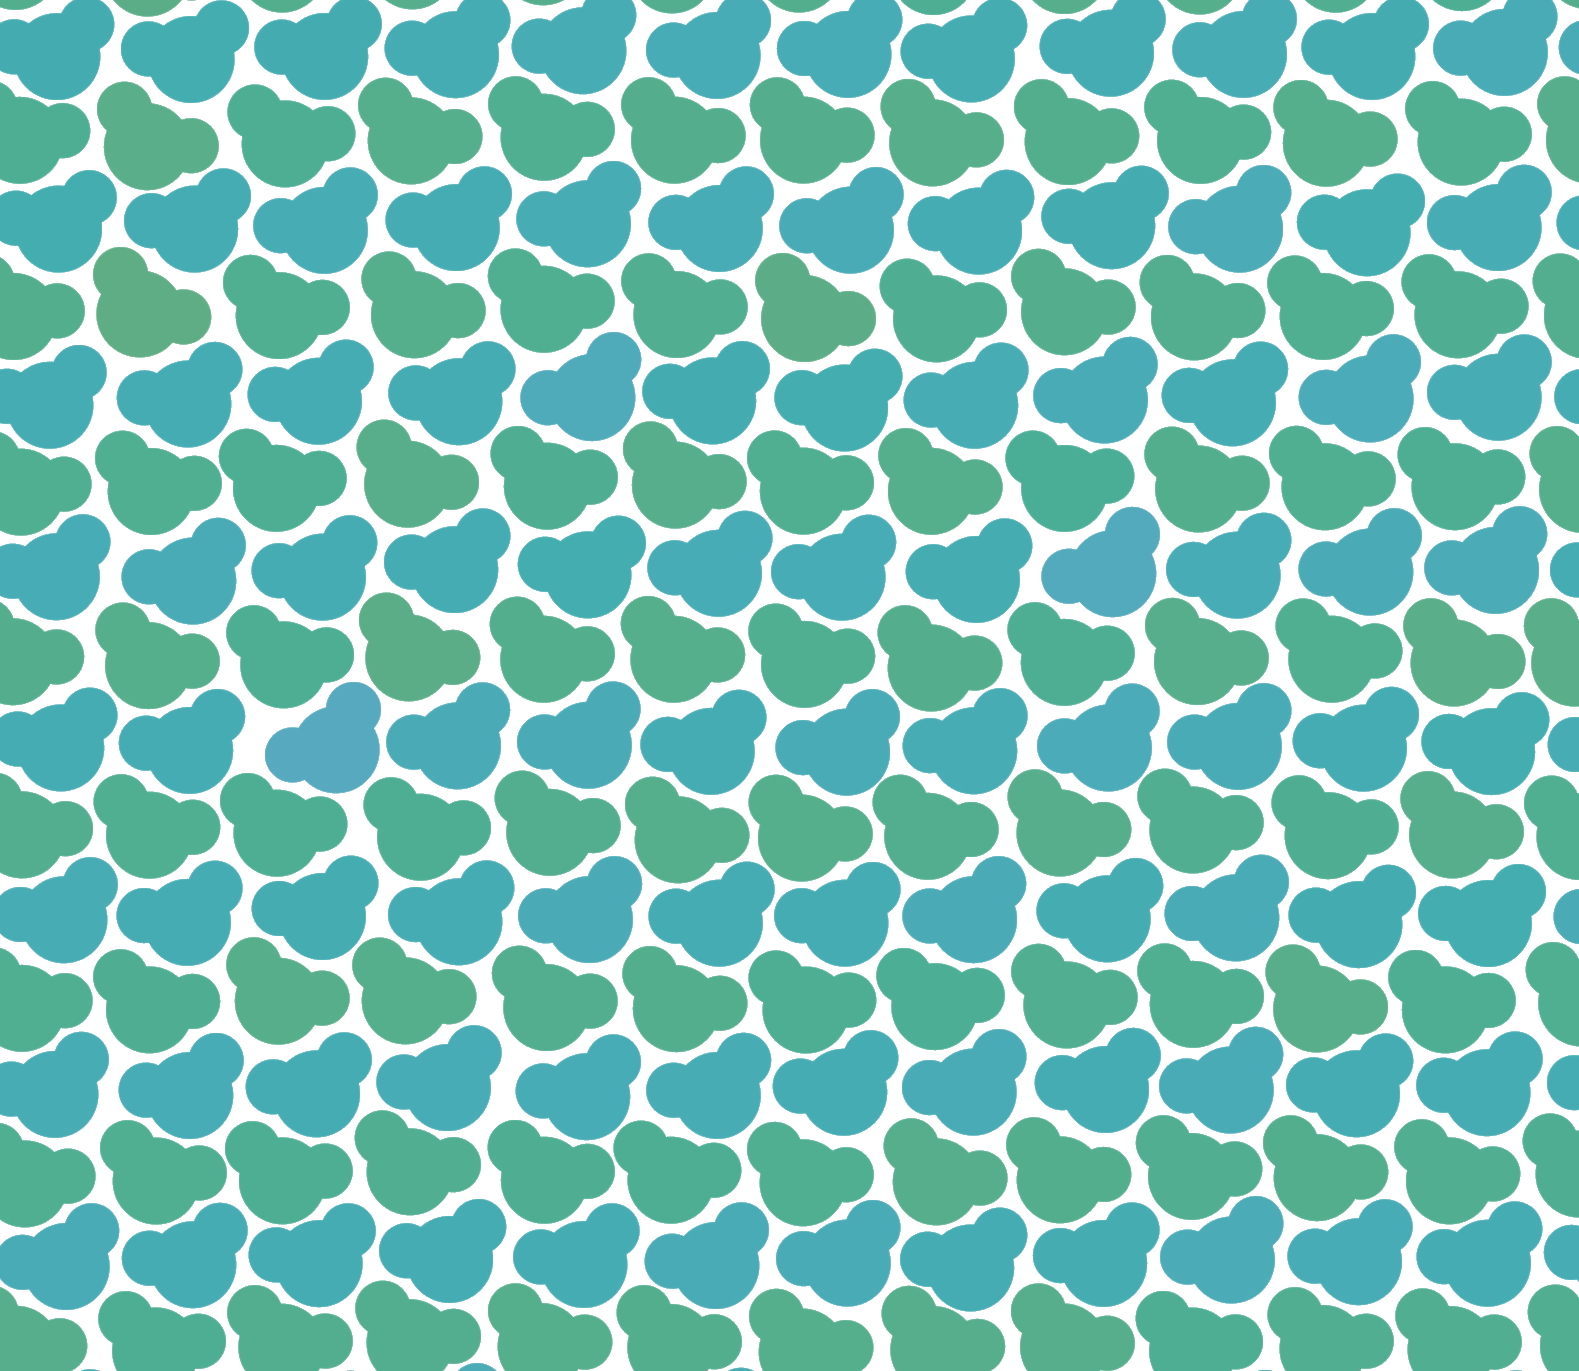
\includegraphics[width=\linewidth]{trimer-crys-pg}
            \caption{pg}
            \label{fig:crystals pg}
          \end{subfigure}
          \begin{subfigure}[t]{0.3\linewidth}
              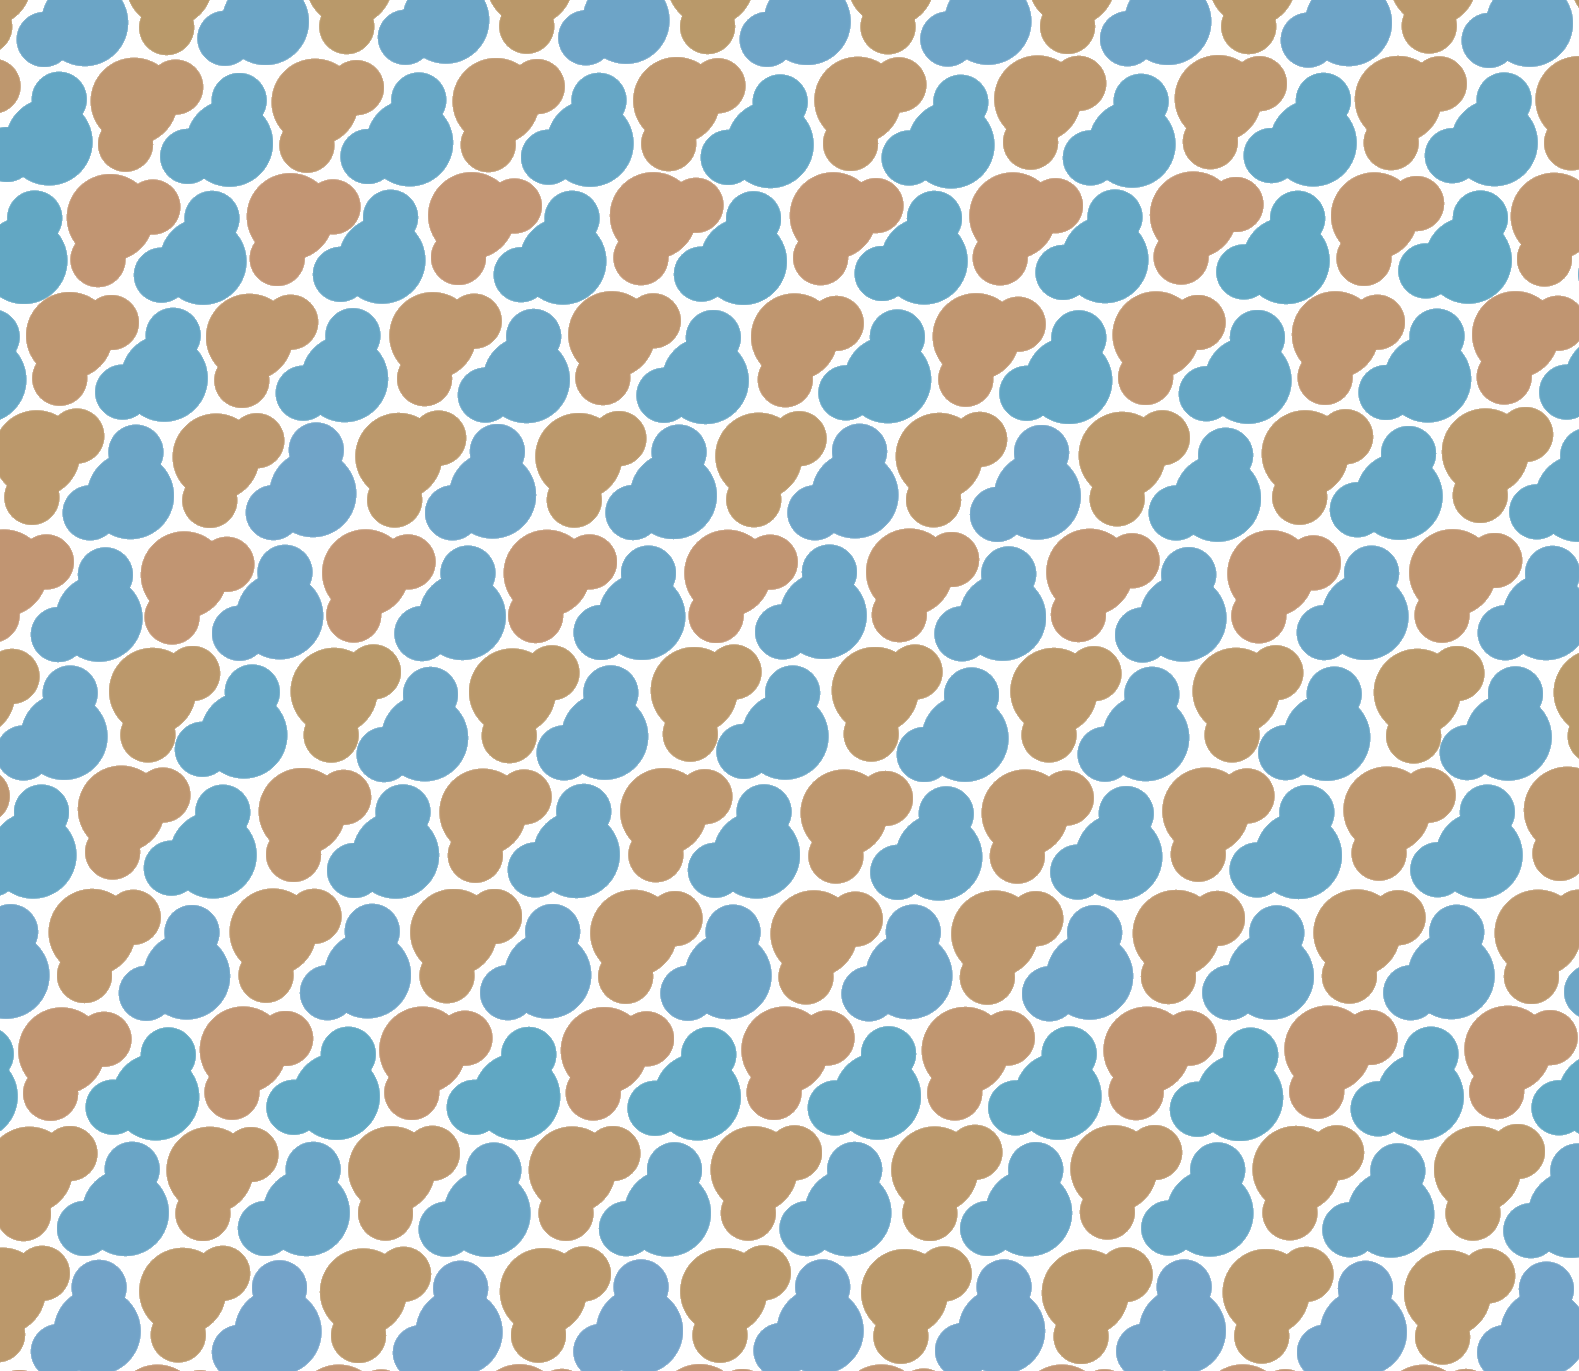
\includegraphics[width=\linewidth]{trimer-crys-p2}
            \caption{p2}
            \label{fig:crystals p2}
          \end{subfigure}
          \begin{subfigure}[t]{0.3\linewidth}
              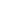
\includegraphics[width=\linewidth]{trimer-crys-p2gg}
            \caption{p2gg}
            \label{fig:crystals p2gg}
          \end{subfigure}
          \caption{The three lowest energy structures of the Trimer molecule}
          \label{fig:crystals}
        \end{figure}
        These structures have very different configurations making it
        difficult to detect all of them with a single metric.

      \end{block}

    \begin{block}{Machine Learning Methodology}
      The orientation of the crystals is very different between the crystals structures,
      and is highly disordered in the liquid phase hence was chosen as the feature
      for machine learning.

      \begin{figure}[h]
        \centering
        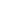
\includegraphics[width=0.8\linewidth]{orientations}
        \caption{Taking the relative orientations of the nearest neighbours.}
        \label{fig:orientations}
      \end{figure}


    \end{block}

    \begin{block}{References}

    \end{block}

    \end{column}
    \begin{column}{0.45\linewidth}
      \begin{block}{Results}

        \begin{figure}[h]
          \centering
          \begin{subfigure}[t]{\linewidth}
              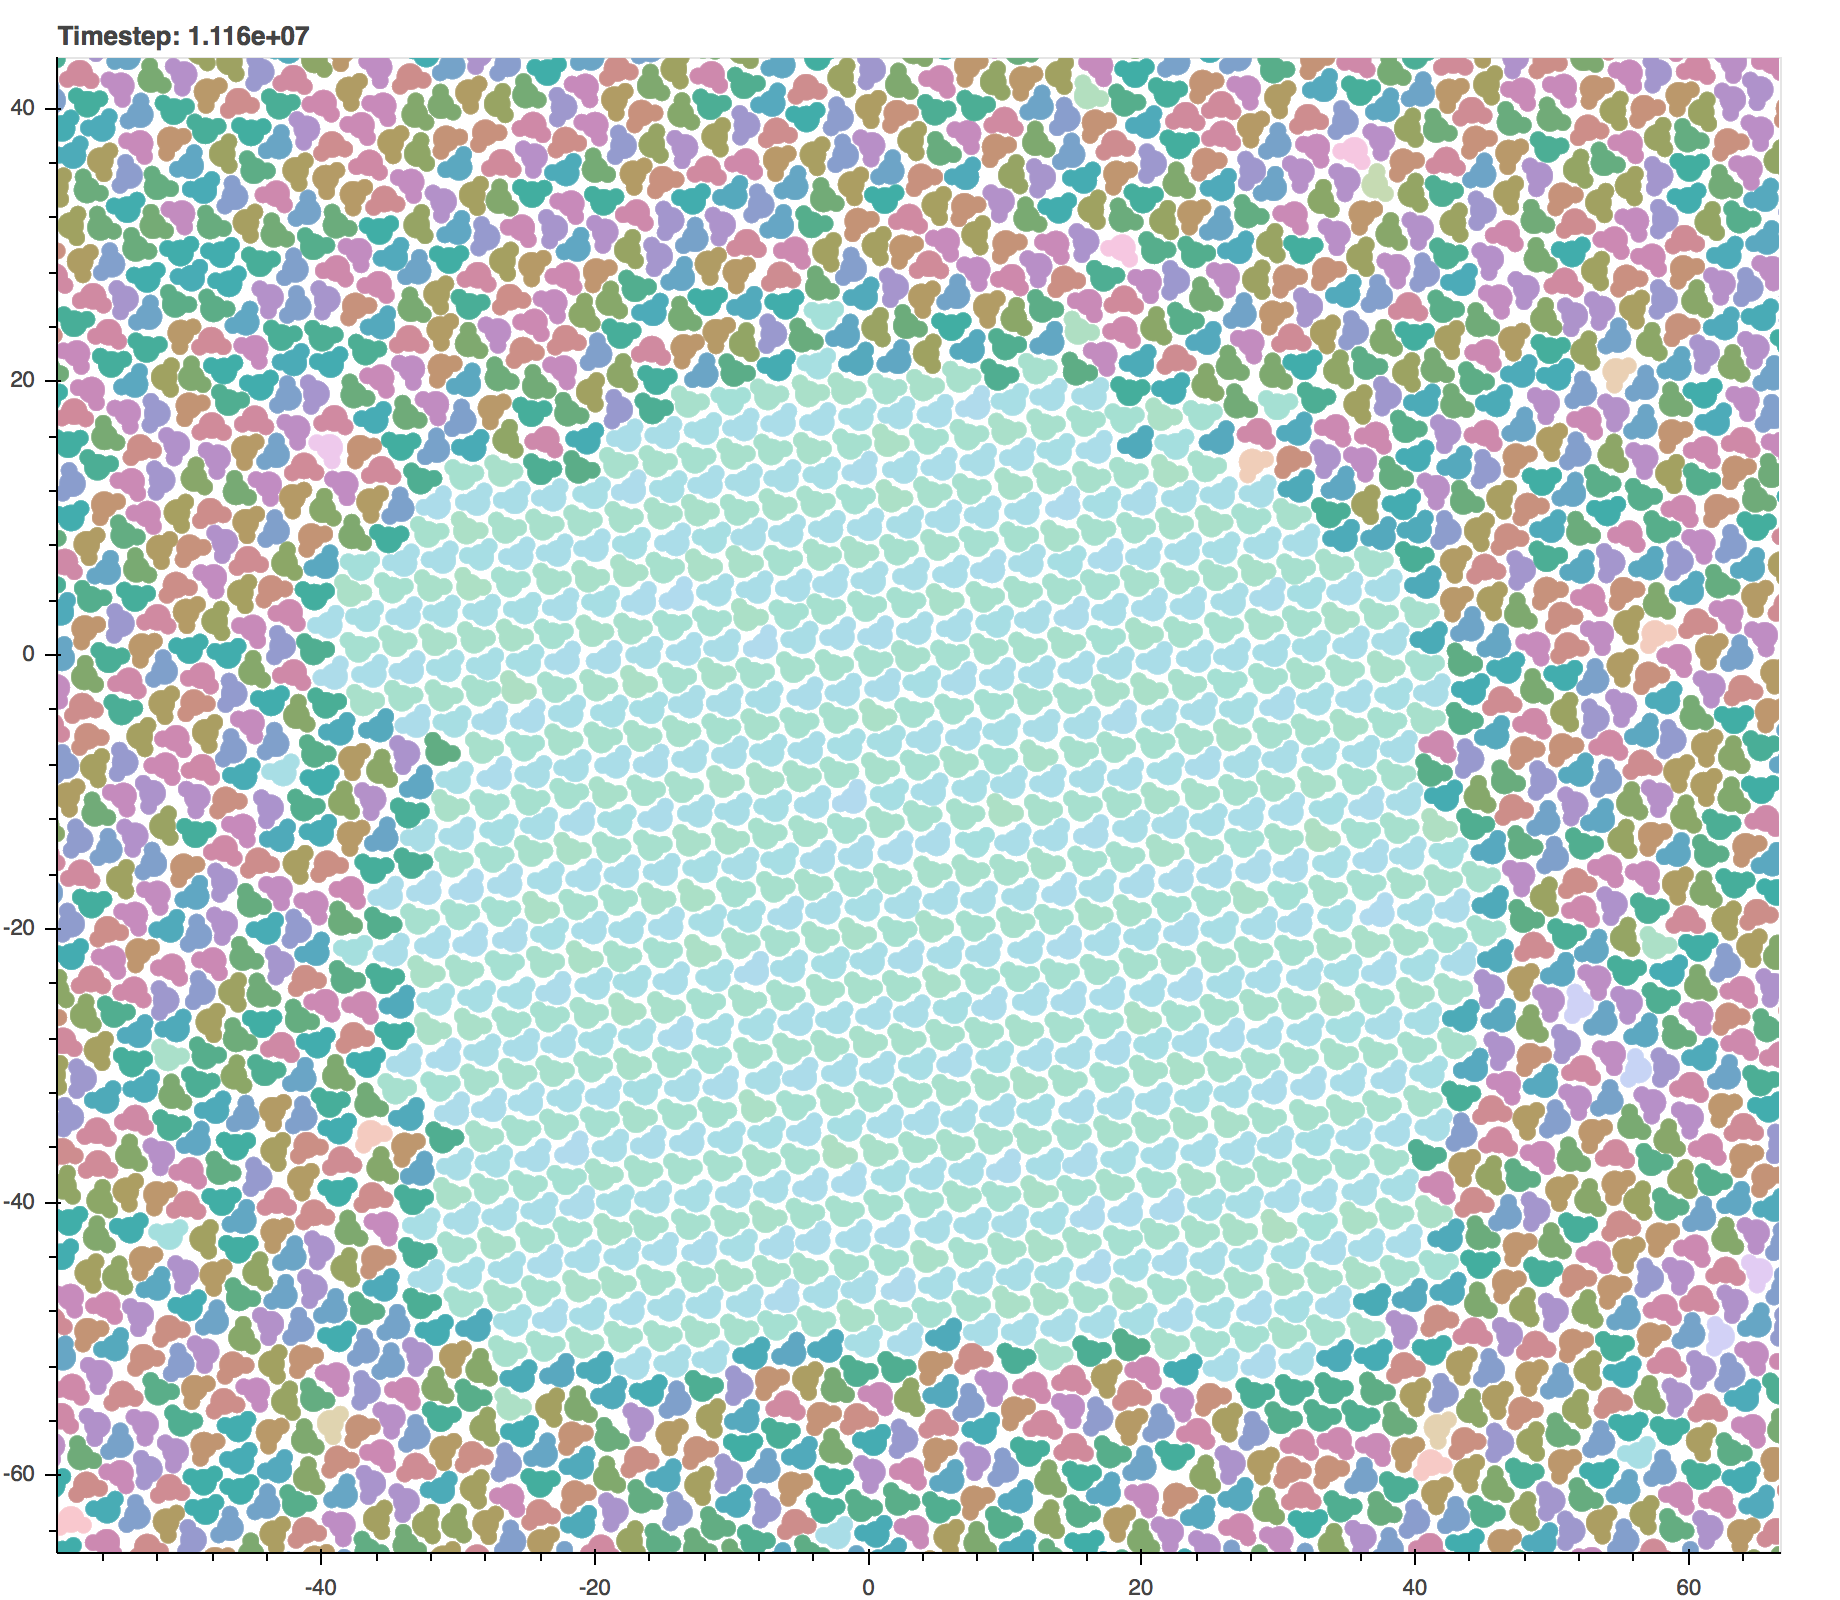
\includegraphics[width=0.5\linewidth]{trimer-cat-pg}
            \caption{pg}
            \label{fig:categorised pg}
          \end{subfigure}
          \begin{subfigure}[t]{\linewidth}
              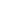
\includegraphics[width=0.5\linewidth]{trimer-cat-p2}
            \caption{p2}
            \label{fig:categorised p2}
          \end{subfigure}
          \begin{subfigure}[t]{\linewidth}
              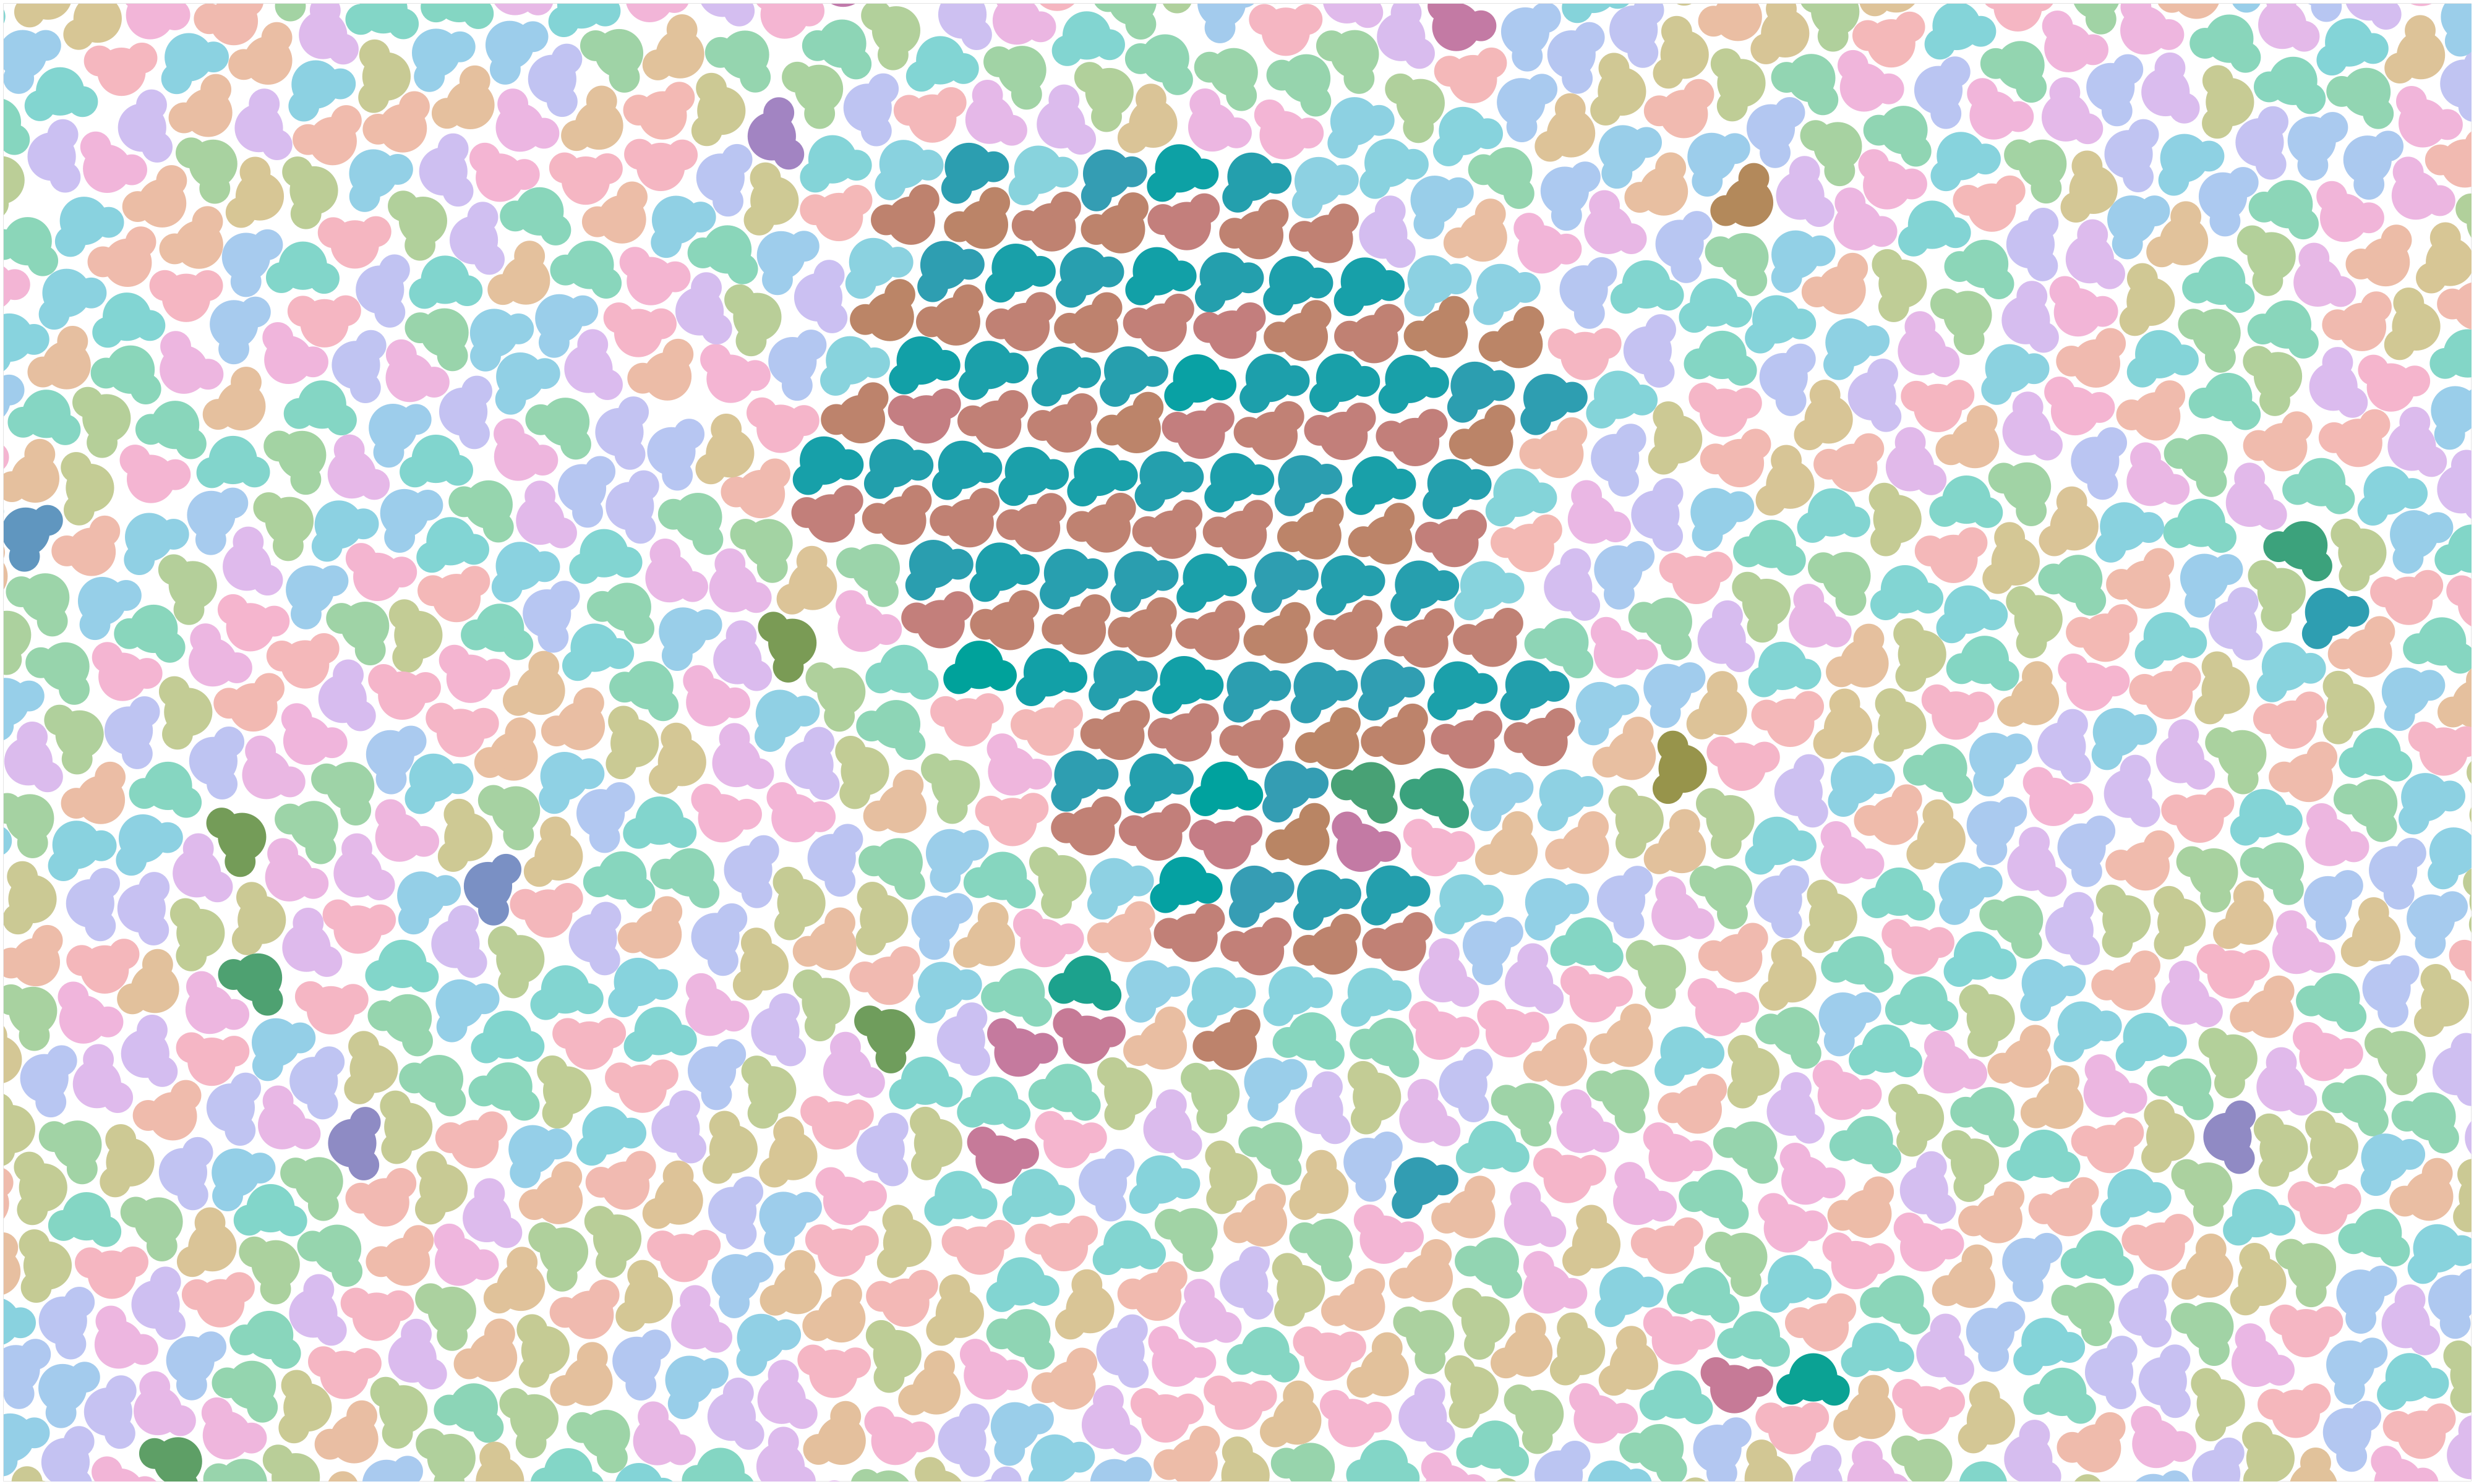
\includegraphics[width=0.5\linewidth]{trimer-cat-p2gg}
            \caption{p2gg}
            \label{fig:categorised p2gg}
          \end{subfigure}
          \caption{Each of the crystal structures characterised using the same
          machine learning algorithm}
          \label{fig:categorised}
        \end{figure}


        %This can be used to compute a melting rate
        %\begin{figure}[h]
          %\centering
          %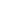
\includegraphics[width=0.8\linewidth]{trimer-melting}
          %\caption{Melting of the Trimer crystals}
          %\label{fig:melting}
        %\end{figure}
      \end{block}

      \begin{block}{Future Work}
        I would like to extend this work to the
        generalised characterisation of 3D molecular crystals.
        At the current stage I am lacking the datasets of
        liquid an crystal configurations to test this out.
      \end{block}

    \end{column}
  \end{columns}
\end{frame}

\end{document}
